\documentclass[a4paper,12pt]{report}
\usepackage{cmap}		
\usepackage[utf8]{inputenc}
\usepackage{framed}
\usepackage[english,russian]{babel}
\usepackage{framed}
\usepackage{hyperref}
\usepackage{amsmath}
\usepackage{graphicx}
\usepackage[colorinlistoftodos]{todonotes}
\usepackage{wrapfig}
\usepackage{lipsum}
\usepackage{listings}
\usepackage{color}
\usepackage{indentfirst}
\usepackage{times}
\usepackage{textcomp}
\usepackage{wrapfig}
\usepackage{adjustbox}
\usepackage{txfonts}
\usepackage{lipsum}
\usepackage{physics}
\usepackage{rotating}

\usepackage{listings}

\graphicspath{{../}}

\definecolor{mygray}{rgb}{0.4,0.4,0.4}
\definecolor{mygreen}{rgb}{0,0.8,0.6}
\definecolor{myorange}{rgb}{1.0,0.4,0}
\definecolor{codegreen}{rgb}{0,0.6,0}
\definecolor{codegray}{rgb}{0.5,0.5,0.5}
\definecolor{codepurple}{rgb}{0.58,0,0.82}
\definecolor{backcolour}{rgb}{0.95,0.95,0.92}

\lstdefinestyle{customc}{
	% backgroundcolor=\color{backcolour},
	belowcaptionskip=1\baselineskip,
	breaklines=true,
	frame=L,
	xleftmargin=\parindent,
	language=sh,
	showstringspaces=false,
	basicstyle=\ttfamily\bfseries,
	columns=fixed,
	morekeywords={ifconfig,ip,route,dhclient,nmcli,ping},
	keywordstyle=\bfseries\color{green!40!black},
	commentstyle=\itshape\color{purple!40!black},
	identifierstyle=\color{blue},
	stringstyle=\color{purple},
	numbers=left,
	numbersep=12pt,
	numberstyle=\ttfamily\scriptsize\color{mygray},
	tabsize=2,
}
\lstset{style=customc}




\newcommand{\HRule}{\rule{\linewidth}{0.5mm}}

\begin{document}
	
	\begin{titlepage}
	\begin{center}
		
		\textsc{\Large Федеральное государственное автономное образовательное учреждение высшего образования}\\
		\textsc{\large "Национальный исследовательский университет ИТМО"}\\[0.5cm]
		
		% Upper part of the page. The '~' is needed because \\
		% only works if a paragraph has started.
		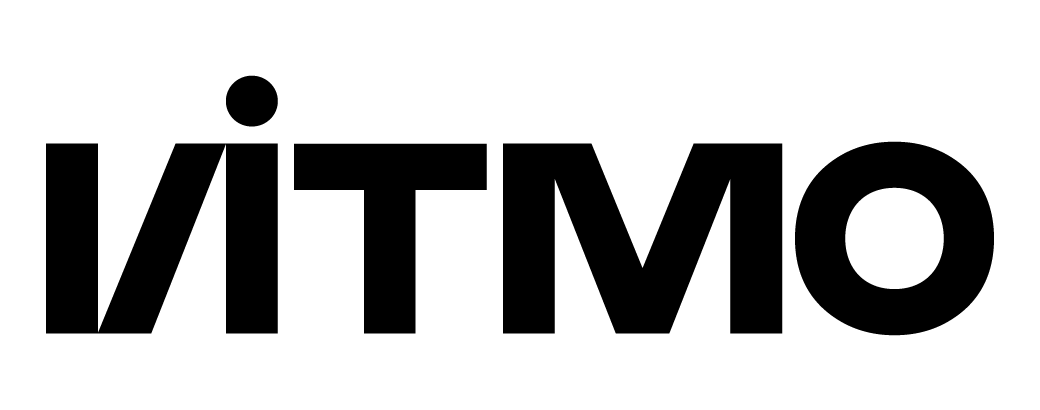
\includegraphics[width=0.5\textwidth]{img/logo.png}~\\[0.5cm]
		
		\textsc{\Large Факультет информационных технологий и программирования\ \\ Отчет по лабораторной работе №3 \\ "Работа с \LaTeX"\\[5cm]}
		
		
		% Author and supervisor
		\noindent
		\begin{minipage}{0.4\textwidth}
			\begin{flushleft} \large
				\emph{Выполнил:}\\
				Гильмутдинов \textsc{А.Р.}, М3116
			\end{flushleft}
		\end{minipage}
		\begin{minipage}{0.4\textwidth}
			\begin{flushright} \large
				\emph{Преподаватель:}\\
				\quad\quad\quadХасан\ \textsc{К.А.}
			\end{flushright}
		\end{minipage}
		
		\vfill
		
		% Bottom of the page
		{\large Октябрь 2024}
		
	\end{center}
\end{titlepage}
	
	\newpage
	\tableofcontents
	
	
	\begin{framed}
		\noindent Цель работы:
		\begin{tabbing}
			Cоставить описание библиотеки \verb|geometric_lib| в формате PDF \\
			с помощью "\LaTeX";
		\end{tabbing}
		
	\end{framed}
	
	
	\newpage
	\section{Общее описание библиотеки geometric lib}
	
	В ветке develop находятся четыре python файла:
	\begin{itemize}
		\item calculate.py - выполняет функцию подсчета периметра или площади заданной фигуры;
		\item circle.py - содержит функции подсчета периметра и площади круга.
		\item square.py - содержит функции подсчета периметра и площади квадрата.
		\item triangle.py - содержит функцим подсчета периметра и площади треугольника.
	\end{itemize}
	
	
	
	\newpage
	\section{Описание исходных файлов библиотеки}
	
	\begin{enumerate}
		\item calculate.py: 
		
			\begin{lstlisting}
				import circle
				import square
				
				
				figs = ['circle', 'square']
				funcs = ['perimeter', 'area']
				sizes = {}
				
				def calc(fig, func, size):
					assert fig in figs
					assert func in funcs
					
					result = eval(f'{fig}.{func}(*{size})')
					print(f'{func} of {fig} is {result}')
					
				if __name__ == "__main__":
					func = ''
					fig = ''
					size = list()
				
					while fig not in figs:
						fig = input(f"Enter figure name, avaliable are {figs}:\n")
					
					while func not in funcs:
						func = input(f"Enter function name, avaliable are {funcs}:\n")
					
					while len(size) != sizes.get(f"{func}-{fig}", 1):
						size = list(map(int, input("Input figure sizes separated by space, 1 for circle 	and square\n").split(' ')))
				
					calc(fig, func, size)
			\end{lstlisting}
	
			\newpage
			
			В заголовке файла:
			\begin{itemize}
				\item Импорт необходимых файлов для расчета площади и периметра для фигур.
				\item Инициализация массивов, содержащих возможные параметры для функции calc.
			\end{itemize}
			
			
			В main'е файла:
			\begin{itemize}
				\item Инициализация переменных, необходимых для функции calс.
				\item Пользовательский ввод данных и Проверка их на валидность.
				 	  Цикл "while" не даёт возможности ввести некорректные данные.
				\item Вызов функции calc.
			\end{itemize}
		
			В функции calc файла:
			\begin{itemize}
				\item Фунция calc в качестве аргументов принимает: название фигуры, фунции,
					  длину стороны квадрата или радиус круга.\\
				 	  Возращает значение, полученное при выполнении функции, находящейся в
				 	  поле данной фигуры.\\
					  Выводит в консоль результат. 
			\end{itemize}
			
			\newpage
			
		\item circle.py:
			\begin{lstlisting}
				import math
				
				def area(r):
					return math.pi * r * r
				
				def perimeter(r):
					return 2 * math.pi * r
			\end{lstlisting}
			\begin{itemize}
				\item Импорт библиотеки "math", чтобы использовать $\pi$;
				\item Фунция "area" возвращает площадь круга,\\ принимает радиус аргументом.\\
					  $S = \pi r^2$
				\item Функция "perimeter" возвращает периметр круга,\\ принимает радус аргументом.\\
					  $S = 2 \pi r$
			\end{itemize}
			
		\item square.py:
			\begin{lstlisting}
				def area(a):
					return a * a
				
				def perimeter(a):
					return 4 * a
			\end{lstlisting}
			\begin{itemize}
				\item Фунция "area" возвращает площадь квадрата,\\ принимает размер стороны аргументом.\\
					  $S = a^2$
				\item Функция "perimeter" возвращает периметр квадрата,\\ принимает размер стороны аргументом.\\
				      $P = 4a$
			\end{itemize}
			
		\newpage
			
		\item triangle.py:
		\begin{lstlisting}
			def area(a, b, c):
				return (a + b + c) / 2
			
			def perimeter(a, b, c):
				return a + b + c
		\end{lstlisting}
		\begin{itemize}
			\item Фунция "area" возвращает площадь треугольник,\\ принимает размеры трех сторон аргументами.\\
				  $S = \frac{a + b + c}{2}$
			\item Функция "perimeter" возвращает периметр треугольник,\\ принимает размеры трех сторон аргументами.\\
				  $P = a + b + c$
		\end{itemize}
	\end{enumerate}
	
	
	\newpage
	\section{Ссылка на GitHub}
	Ссылка на GitHub с исходным кодом данной документации в \LaTeX: \href{https://github.com/argilmutdinov/ISRPO_LaTeX_lab}{GitHub}
	
	
	
	
	
	
	
	
	
	
	
	
	
	
	
	
	
	
\end{document}